\chapter{Ralentissements des neutrons}
\section{Introduction}
La diminution de l'énergie des neutrons de $E_{fission}$ à $E_{th}$ peut se faire par scattering 
élastique ou inélastique. Regardons les deux cas
\begin{enumerate}
\item \textit{Collisions inélastiques} :: l faut que l'énergie du neutron incident soit supérieur au 
premier niveau d'excitation du noyau. Celui ci vaut
\begin{itemize}
\item[$\bullet$] 1 MeV pour les noyaux légers
\item[$\bullet$] 0.1 MeV pour les noyaux lourds
\end{itemize}
Les collisions inélastiques avec des noyaux lourds sont possibles, mais pour des valeurs d'énergie
bien supérieures au domaine de résonance.
\item \textit{Collisions élastiques} : celle-ci n'est pas efficace avec les noyaux lourds et il faut
dès lors utiliser des noyaux légers, qui joueront le rôle de \textit{modérateurs}.
\end{enumerate}

\section{Ralentissement via scattering inélastique}
\subsection{Cinématique}
	\begin{wrapfigure}[11]{l}{10cm}
	\vspace{-5mm}
	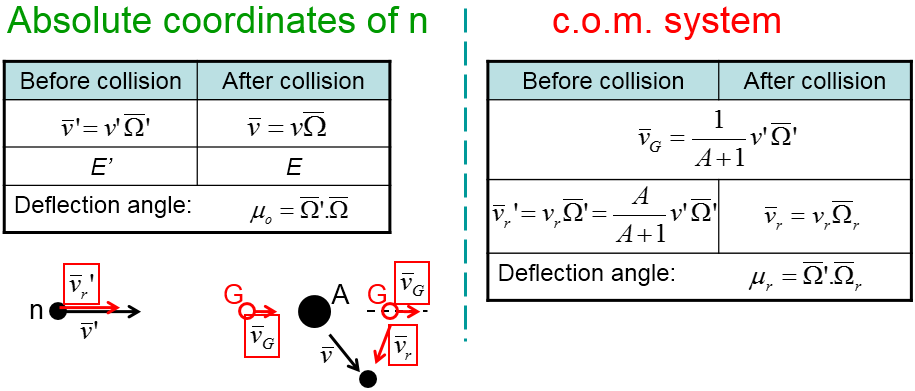
\includegraphics[scale=0.4]{ch7/image1.png}
	\captionof{figure}{ }
	\end{wrapfigure}
	Le but est d'étudier l'effet des collisions élastiques sur le ralentissement. Dans le système de 
	coordonnées \textit{absolue}, le neutron est initialement caractérisé par $\bar v'$ et $E'$ avant 
	collision et après par $\bar v$ et $E$. Dans le système du \textit{centre de masse}, il faut 
	considérer une vitesse relative avant la collision\footnote{$A$ est la masse du noyau et 1 la
	masse du neutron, on comprend alors le sens du dénominateur servant à la pondération.}. Par 
	collision élastique, la vitesse relative possède une amplitude similaire à la situation avant 
	collision mais une direction modifiée. \\
	
	La vitesse du centre de masse et celle du neutron sont donc conservée dans le mouvement relatif
	mais il y a modification de la direction.\\
	
	La vitesse, étant relative, est donnée par la somme de la vitesse du centre de masse $\bar v_G$ et 
	la vitesse relative $\bar v_r$
	\begin{equation}
	\bar v = {\bar v_G} + {\bar v_r} = \frac{{v'}}{{A + 1}}(\bar \Omega ' + A{\bar \Omega _r})
	\end{equation}
	En prenant les modules carré de part et d'autre et que l'on effectue le ratio de l'énergie 
	finale sur l'énergie incidente, on trouve
	\begin{equation}
	\frac{E}{{E'}} = \frac{{{v^2}}}{{v{'^2}}} = \frac{{{A^2} + 2A{\mu _r} + 1}}{{{{(A + 1)}^2}}}
	\end{equation}
	
	\begin{wrapfigure}[7]{r}{2.5cm}
	\vspace{-5mm}
	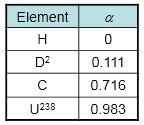
\includegraphics[scale=0.7]{ch7/image2.png}
	\captionof{table}{ }
	\end{wrapfigure}
	La seule chose pouvant varier dans cette expression est $\mu_r$ (il contient le cosinus de l'angle
	entre la direction d'entrée et de sortie). Comme cosinus est majoré par 1 et minoré par zéro, 
	on peut trouver un minimum d'énergie
	\begin{equation}
	{E_{\min }} = {\left( {\frac{{A - 1}}{{A + 1}}} \right)^2}E' \equiv \alpha \,E'
	\end{equation}
	La valeur $\alpha$ permet d'avoir un ordre de grandeur pour le ralentissement. L'hydrogène 
	fera ainsi un bon modérateur. Par contre si l'on veut ralentir l'$U^{238}$, il ne faut pas 
	être trop pressé.\\
	
	Il existe plusieurs relations entres les variables:
	\begin{itemize}
	\item[$\bullet$] $\mu_0=f(\mu_r)$ ; on utilise le rapport $v'/v$ avec le rapport des énergies (
	racine de l'inverse, où $\mu_r$ est la déflection angulaire dans le système absolu)
	\begin{equation}
	{\mu _o} = \frac{1}{v}\bar v.\bar \Omega ' = \frac{1}{v}\frac{{v'}}{{A + 1}}(\bar \Omega ' +
	 A{\bar \Omega _r}).\bar \Omega '  = \frac{1}{{A + 1}}\sqrt {\frac{{E'}}{E}} (A{\mu _r} + 1)
	 \Rightarrow  \to \;{\mu _o} = \frac{{A{\mu _r} + 1}}{{\sqrt {{A^2} + 2A{\mu _r} + 1} }}
	\end{equation}
	\item[$\bullet$] ${\mu _r} = f(E)$ ; inverse de l'expression ci-dessus (où $\mu_r$ est la 
	déflection angulaire dans le système du centre de masse)
	\begin{equation}
	{\mu _r} = \frac{{{{(A + 1)}^2}}}{{2A}}\frac{E}{{E'}} - \frac{{{A^2} + 1}}{{2A}}
	\end{equation}
	\item[$\bullet$] $\mu_0 = F(E)$ ; défini sur base des énergies
	\begin{equation}
	{\mu _o} = \frac{{A + 1}}{2}\sqrt {\frac{E}{{E'}}}  - \frac{{A - 1}}{2}\sqrt {\frac{{E'}}{E}} 
	\end{equation}
	\item[$\bullet$] ${\mu _r} = f({\mu _o})$
	\begin{equation}
	{\mu _r} = \frac{1}{A}(\mu _o^2 + {\mu _o}\sqrt {{A^2} - 1 + \mu _o^2}  - 1)
	\end{equation}
	\end{itemize}
	En laboratoire, on mesurera $\mu_0$ ($\mu_r$ est exprimé dans le référentiel du centre de 
	masse).
	
	\subsection{Loi de scattering}
	Il s'agit d'une fonction de densité de probabilité (\textit{pdf}) de l'angle de déflexion. 
	Celle-ci est habituellement donnée pour le système du centre de masse. Si le scattering 
	est isotrope (centre de masse)
	\begin{equation}
	p({\mu _r})d{\mu _r} = \frac{1}{2}d{\mu _r}
	\end{equation}
	où le facteur $1/2$ vient du $d\cos\theta$ dans l'élément d'angle solide. Ce qui nous intéresse, 
	c'est le mouvement observé au laboratoire. Grâce à la relation
	\begin{equation}
	p({\mu _r})d{\mu _r} = p({\mu _o})d{\mu _o}
	\end{equation}
	On peut écrire (en utilisant les relations entre variables décrites ci-dessus)
	\begin{equation}
	p({\mu _o}) = \frac{1}{{2A}}\left(   \frac{{{A^2} - 1 + 2\mu _o^2}}{{\sqrt {{A^2} - 1 +
	\mu _o^2} }} + 2{\mu _o}  \right) \quad\overset{A \gg 1}{\longrightarrow}\quad \frac{1}{2}
	\end{equation}
	Pour une masse de noyau tendant vers l'infini, on retrouve une densité de probabilité constante
	valant $1/2$. Ce résultat était attendu car si les masses tendent vers l'infini, il n'y a plus 
	de différence entre le mouvement absolu et relatif\footnote{Le "facteur de pondération" tend 
	vers $1/2$.}.\\
	
	Dans le cas où $A=1$
	\begin{equation}
	p({\mu _o}) = |{\mu _o}| + {\mu _o} = \left\{ {\begin{array}{*{20}{c}}
	{2{\mu _o}}&{si\,{\mu _o} > 0}\\
	0&{si\,{\mu _o} < 0}
	\end{array}} \right.
	\end{equation}
	Ceci ne concerne que le scattering vers l'\textit{avant}, il n'y a donc \textit{aucune} 
	rétro-diffusion ici\footnote{Limite du modèle ou réalité physique?}.\\
	
	On défini le \textbf{noyau de ralentissement} comme étant la fonction de densité de probabilité 
	de l'énergie d'un neutron ayant subit un scattering dans le cas isotropique. Sachant 
	que\footnote{Justif?} $K(E|E')dE = p({\mu _r})d{\mu _r}$, on trouve\\
	
	\cadre{\begin{equation}
	K(E|E') = \left\{ {\begin{array}{*{20}{c}}
	{\dfrac{1}{{(1 - \alpha )E'}}}&{if\,\alpha E' \le E \le E'}\\
	0&{else}
	\end{array}} \right.
	\end{equation}}\ \\
	
	On notera que le fait d'avoir un scattering isotrope dans le mouvement du centre de masse 
	n'implique pas que ce-dernier le soit également dans le mouvement absolu : quelque chose qui 
	va de l'avant peut être vu comme isotrope d'un point de vue relatif.\\
	
	De par la relation $K(E|E')dE = p({\mu _r})d{\mu _r}$, il est possible de calculer la \textit{
	perte d'énergie moyenne par collision élastique}\\
	
	\cadre{\begin{equation}
	 < E' - E >  = \int_{\alpha E'}^{E'}    (E' - E)K(E|E')dE = \frac{{(1 - \alpha )E'}}{2}
	\end{equation}}\ \\
	
	\begin{wrapfigure}[5]{r}{2.5cm}
	\vspace{-5mm}
	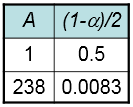
\includegraphics[scale=0.7]{ch7/image3.png}
	\captionof{table}{ }
	\end{wrapfigure}
	La valeur moyenne se trouve logiquement au centre de l'intervalle des énergies. Cette valeur 
	moyenne augmente avec $E'$ mais diminue avec $A$ car 
	\begin{equation}
	\frac{{(1 - \alpha )}}{2} = \frac{{2A}}{{{{(A + 1)}^2}}}
	\end{equation}

\newpage

	\subsection{Lethargie}
	\textit{Quoi de mieux qu'un lundi matin pour introduire une nouvelle variable énergie ?} En 
	effet, les dernières constatations poussent à introduire cette grandeur qui a \textit{augmente} 
	lorsque les neutrons \textit{ralentissent}\ \\
	
	\cadre{\begin{equation}
	u = \ln \frac{{{E_o}}}{E}
	\end{equation}
	Étant par définition positive, on en tire la valeur de l'état de référence $E_{ref}=E_0 : 
	u > 0 \forall E \to E_0 = 10\ $MeV.}\ \\
	
	Le but d'introduire cette variable est de pouvoir ré-écrire le noyau de ralentissement en 
	fonction de la lethargie $K(u|u')du = K(E|E')dE$. Pour se faire, il faut que\footnote{Pour 
	la suite, on défini $\ln\frac{1}{\alpha}\equiv q$.}
	\begin{equation}
	K(u|u')du = K(E|E')dE  = \frac{{{e^{ - (u - u')}}}}{{1 - \alpha }}du
	\end{equation}
	où $\alpha E' \le E \le E'\; \Rightarrow \;u' \le u \le u' + \ln \frac{1}{\alpha }$. Ceci 
	étant défini on peut faire le même raisonnement que pour l'énergie et calculer la 
	\textit{lethargie moyenne \textbf{gagnée} par collision élastique}
	\begin{equation}
	\xi  =  < u - u' >  = \int_{u'}^{u' + \ln \frac{1}{\alpha }}   (u - u')K(u|u')du = 1 -
	 \frac{\alpha }{{1 - \alpha }}\ln \frac{1}{\alpha }
	\end{equation}
	"\textit{Il s'agit d'une intégrale qui devrait vous être faisable en quatre jours}". On 
	remarque que ce résultat est \textit{indépendant} de $u'$ ! Le petit tour de passe-passe 
	opéré avec la lethargie est que, avec cette variable, le saut moyen qui va se faire n'est 
	plus qu'une caractéristique du noyau avec lequel il interagit. Après résolution
	\begin{equation}
	\xi  = 1 - \frac{{{{(A - 1)}^2}}}{{2A}}\ln \frac{{A + 1}}{{A - 1}}
	\end{equation}
	Avec un gain moyen en lethargie unitaire ($\xi=1$) pour l'hydrogène ($A=1$). Le point vraiment
	fondamental est que chaque collision, en moyenne, est une caractéristique de l'élément cible 
	indépendamment de l'énergie de départ et en plus la référence hydrogène correspond à un gain
	de 1, si c'est pas beau ça ! Le nombre moyen de collisions pour une augmentation de léthargie
	donnée est de
	\begin{equation}
	\Delta u = n\xi
	\end{equation}
	Ceci signifie que pour traverser une intervalle de lethargie $\Delta u$, il est nécessaire 
	de subir $n$ collisions pour traverser cet intervalle. \\
	
	\begin{wrapfigure}[8]{l}{9.5cm}
	\vspace{-8mm}
	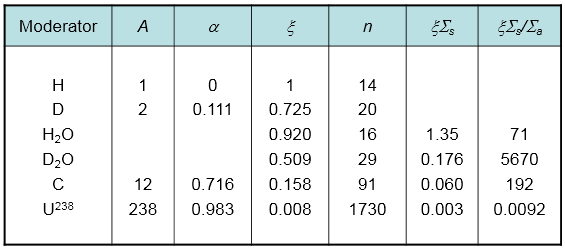
\includegraphics[scale=0.6]{ch7/image4.png}
	\captionof{table}{ }
	\end{wrapfigure}
	Ces grandeurs permettent de définir ce qu'est un modérateur efficace. Un bon modérateur présente
	un gain moyen en lethargie par collision le plus élevé que possible mais ce n'est pas 
	suffisant : il faut également avoir suffisamment de scattering sinon rien ne sera ralenti. 

	\newpage 
	On défini alors le \textbf{pouvoir de modération}
	\begin{equation}
	\text{Pouvoir de modération }: \quad \xi\Sigma_s
	\end{equation}
	Il faut que ce pouvoir de modération soit important, mais également l'absorption la plus faible
	que possible. On défini alors le \textbf{ratio de modération}
	\begin{equation}
	\text{Ratio de modération }: \quad \xi\Sigma_s/\Sigma_a		
	\end{equation}
	Le tableau en bas de la précédente page reprend les différents paramètres nous permettant de 
	choisir un \textit{bon} modérateur. 


	\subsection{Section efficace différentielle}
	Le lien entre la section efficace différentielle et la section totale de scattering est fait par
	le noyau de ralentissement\\
	
	\cadre{\begin{equation}
	{\Sigma _s}(\bar r,u' \to u) = {\Sigma _s}(\bar r,u')K(u|u')
	\end{equation}}\ \\
	
	On peut exprimer la section efficace différentielle en terme de lethargie et d'angles
	\begin{equation}
	{\Sigma _s}(\bar r,u',\bar \Omega ' \to u,\bar \Omega ) = {\Sigma _s}(\bar r,u')K(u|u')\frac{1}
	{{2\pi }}f({\mu _o})
	\end{equation}
	Comme précédemment, le cosinus de l'angle de déflection est déterminé par la cinématique des 
	collisions élastiques
	\begin{equation}
	{\mu _o} = \frac{{A + 1}}{2}\sqrt {\frac{E}{{E'}}}  - \frac{{A - 1}}{2}\sqrt {\frac{{E'}}{E}} 
	{\mu _o} = \frac{{A + 1}}{2}\sqrt {\frac{E}{{E'}}}  - \frac{{A - 1}}{2}\sqrt {\frac{{E'}}{E}} 
	\end{equation}
	On obtient une combili d'exponentielles contenant un delta en lethargie. Il en vient que
	\footnote{?}
	\begin{equation}
	f({\mu _o}) = \delta ({\mu _o} - {\mu _o}(u - u'))
	\end{equation}
	La facteur donnant la déflection angulaire est un delta de Dirac : un pic de variation correspond
	à \textbf{une} déflection angulaire: une variation donnée $\leftrightarrow$ une variation de 
	la lethargie.


\section{Équation de ralentissement}
	\subsection{Approximation $P_1$}
	L'objectif du ralentissement des neutrons est de déplacer le spectre d'énergie des neutrons dans 
	le domaine des collisions élastiques : la diffusion multi-groupe est nécessaire\footnote{On 
	cherche l'expression d'une loi de ralentissement permettant d'adapter le terme source.} et il faut
	prendre en compte les variations spatiales et d'énergie. \textit{Or}, nous n'avons pas de 
	variation spatiale du flux et donc pas de courant impliquant qu'il n'y a pas de diffusion ! Il 
	est dès lors possible de traiter la dépendance spatiale plus simplement.
	
	\subsubsection{Équation de Bolztmann stationnaire en lethargie}	
	Précédemment dans le cours de \textit{Physique des réacteurs nucléaires}, nous avions établi un
	lien entre $D$ et la section efficace (à une vitesse) :
	\begin{equation}
	D = \frac{1}{{3{\Sigma _{tr}}}}\quad\text{où}\quad {\Sigma _{tr}} = {\Sigma _t} -  < {\mu _o} >
	 {\Sigma _s}
	\end{equation}
	On lien avec la déflection angulaire était apparu. Ici, nous avons trouvé que
	\begin{equation}
	p({\mu _o}) = \frac{1}{{2A}}\left( \frac{{{A^2} - 1 + 2\mu _o^2}}{{\sqrt {{A^2} - 1 + \mu _o^2}
	 }} + 2{\mu _o}  \right)
	\end{equation}
	où $\langle\mu_0\rangle \neq 0$ (surtout si $A\approx 1$). Ceci nous donne l'idée de regarder 
	d'un peu plus près l'équation de Boltzmann, "\textit{ce qui n'est pas prendre un risque majeur}",
	écrite cette-fois en terme de lethargie\footnote{On change $v$ en $u$, les dimensions en sont un 
	peu affectées.}
	\begin{equation}
	\begin{array}{ll}
	div\bar J(\bar r,u,\bar \Omega )& \DS + {\Sigma _t}(\bar r,u)\varphi (\bar r,u,\bar \Omega )\\
	 &\DS - \int\limits_{4\pi }    \int_o^u    {\Sigma _s}(\bar r,u',\bar \Omega ' \to
	u,	\bar \Omega )\varphi (\bar r,u',\bar \Omega ')du'd\bar \Omega ' = S(\bar r,u,\bar \Omega )
	\end{array}	\end{equation}	
	Les fissions peuvent venir d'une éventuelle source extérieure donnée par
	\begin{equation}
	\begin{array}{ll}
	S(\bar r,u,\bar \Omega )&\DS = \frac{1}{{4\pi }}\int_{}^{}    {\Sigma _{in}}(\bar r,u' \to u)
	\varphi (\bar r,u')du'\\
	&\DS+ \frac{1}{{4\pi }}\chi (u)\int\limits_{4\pi }   \int_o^u   \nu {\Sigma _f}(\bar r,u')\varphi
	(\bar r,u',\bar \Omega ')du'd\bar \Omega ' + Q(\bar r,u,\bar \Omega )
	\end{array}
	\end{equation}		
	\textit{On va reprendre une vieille connaissance} : l'hypothèse d'anisotropie faible qui nous 
	avait donné le développement du flux suivant
	\begin{equation}
	\varphi (\bar r,u,\bar \Omega ) = \frac{1}{{4\pi }}(\varphi (\bar r,u) + 3\bar \Omega .\bar 
	J(\bar r,u))
	\end{equation}
	En absence de dépendances énergétiques, on va substituer ces équations dans l'équation de 
	Boltzmann et prendre le moment à l'ordre zéro : flux intégrer, plus de dépendance en 
	$\bar{\Omega}$ dans la divergence et la section différentielle ne va plus qu'être fonction 
	de la position et la lethargie :\\
	
	\cadre{
	\begin{equation}
	\int\dots \text{d}\bar\Omega \quad\Rightarrow\quad 
	div\bar J(\bar r,u) + {\Sigma _t}(\bar r,u)\varphi (\bar r,u) - \int_o^u  {\Sigma _s}(\bar r,u'
	\to u)\varphi (\bar r,u')du' = S(\bar r,u)
	\end{equation}}\ \\
	
	Prenons maintenant le moment d'ordre 1. Par isotropie, le membre de droite s'annule lors de 
	l'intégration\\
	
	\cadre{\begin{equation}
	\int\dots \bar\Omega\text{d}\bar\Omega \quad\Rightarrow\quad 	
	\frac{1}{3}\bar \nabla \varphi (\bar r,u) + {\Sigma _t}(\bar r,u)\bar J(\bar r,u) - \int_o^u  
	{\Sigma _{s1}}(\bar r,u' \to u)\bar J(\bar r,u')du' = 0
	\end{equation}
	où ${\Sigma _{s1}}(\bar r,u' \to u) = \int_{\bar \Omega }^{}    {\Sigma _s}(\bar r,u',\bar \Omega
	 ' \to u,\bar \Omega )\bar \Omega '.\bar \Omega d\bar \Omega $.	
	}\ \\
	
	Regardons plus en détail l'expression de $\Sigma_{s1}$. Bien qu'étant le résultat d'une petite
	manipulation, mais il s'agit surtout d'un $\Sigma_s$ avec une dépendance en lethargie. Dans le 
	cas mono-énergétique, nous avons une expression dépendant de la moyenne de la déflection 
	angulaire\footnote{${\Sigma _{tr}} = {\Sigma _t} -  < {\mu _o} > {\Sigma _s}$}. Ici, nous 
	avons $\Sigma_{s,total}$ multiplié par un noyau de scattering et la déflection angulaire, le tout
	multiplié par $\bar{\Omega'}\bar\Omega$. Il s'agit bien de lavaleur moyenne de la déflection 
	angulaire car la distrubtion de cette déflexion est multipliée par cette même déflection : c'est
	la définition de la moyenne statistique. \\
	
	Dans le cas où plusieurs isotopes sont présent, on travaille avec une "mixture" :${\Sigma _s}
	(\bar r,u' \to u) = \sum\limits_i  {\Sigma _{si}}(\bar r,u'){K_i}(u|u')$. On en tire
	\begin{equation}
	{\Sigma _{s1}}(\bar r,u' \to u) = \sum\limits_i  {\Sigma _{si}}(\bar r,u'){K_i}(u|u'){\mu 
	 _{oi}}(u - u')
	\end{equation}
	
	
	\subsection{Densité de ralentissement}	
	Il s'agit du nombre de neutrons (par unité de volume et de temps) ralenti au dessus\footnote{On 
	se rappelle qu'un ralentissement des neutrons cause une augmentation de la léthargie.} d'une 
	lethargie $u$ en un point et direction donnée (version angulaire)\\
	
	\cadre{
	\begin{equation}
	q(\bar r,u,\bar \Omega ) = \int_o^u   \int_{\bar \Omega '}^{}    \left( \int_u^
	\infty     {\Sigma _s}(\bar r,u',\bar \Omega ' \to u,\bar \Omega )du    \right)\varphi
	(\bar r,u',\bar \Omega ')du'd\bar \Omega '
	\end{equation}}\ \\
	
	Il existe aussi une version débarrassée de la partie angulaire que l'on nomme \textbf{densité 
	de ralentissement} (version intégrée donc)\ \\
	
	\cadre{\begin{equation}
	\begin{array}{ll}
	q(\bar r,u) &\DS= \int_o^u   \left(   \int_u^\infty    {\Sigma _s}(\bar r,u' \to u)du
	\right)\varphi (\bar r,u')du'\vspace{2mm}\\
	&=\DS  \int_o^u   \left(  \int_u^\infty     K(u|u')du  \right){\Sigma _s}(\bar r,u')\varphi 
	(\bar r,u')du'
	\end{array}
	\end{equation}}\ \\
	
	On retrouve tout d'abord un terme $\Sigma_s\varphi$ que l'on intègre de 0 à $u$ pour comptabiliser
	les neutrons qui ont une léthargie inférieure à $u$ et qui vont passer au dessus de ce seuil. 
	Ensuite, il faut intégrer sur $du'$ de $u$ à $\infty$ le noyau de ralentissement qui va faire 
	passer les léthargie $u''$ à $u$. De cette façon, on a repris tous les neutrons qui sont ralentis 
	à une léthargie au dessus d'une léthargie donnée. Ce raisonnement est aussi applicable au cas
	angulaire.\\
	
	Il est également possible (à condition d'aimer les intégrales) de définir une \textit{densité de
	courant de ralentissement}
	\begin{equation}
	\begin{array}{ll}
	{\bar q_1}(\bar r,u) &\DS= \int_{\bar \Omega }^{}    \int_o^u    \int_{\bar \Omega '}^{}    \left( 
	\int_u^\infty    {\Sigma _s}(\bar r,u',\bar \Omega ' \to u,\bar \Omega )du  \right)\bar \Omega
	\varphi (\bar r,u',\bar \Omega ')du'd\bar \Omega 'd\bar \Omega\vspace{2mm}\\
	 &\DS = \int_o^u    \left( \int_u^\infty     {\Sigma _{s1}}(\bar r,u' \to u)du  \right)\bar 
	 J(\bar r,u')du'\vspace{2mm}\\
	&\DS= \int_o^u    \left(   \int_u^\infty     K(u|u')du   \right){\Sigma _{s1}}(\bar r,u')\bar
	J(\bar r,u')du'
	\end{array}
	\end{equation}\ \\
	
	Il peut être intéressant d'avoir l'expression de la \textbf{variation de densité de 
	ralentissement}\footnote{\textbf{Interprétation physique manquante!!}}
	\begin{equation}
	\frac{{\partial q(\bar r,u)}}{{\partial u}} = {\Sigma _s}(\bar r,u)\varphi (\bar r,u) - \int_o^u 
	 {\Sigma _s}(\bar r,u' \to u)\varphi (\bar r,u')du'
	\end{equation}
	En prenant le moment au premier ordre, le $\Sigma$ non élastique qui est dans le domaine de
	résonance tend directement vers l'absorption
	\begin{equation}
	div\bar J(\bar r,u) + {\Sigma _{ne}}(\bar r,u)\varphi (\bar r,u) + \frac{{\partial q(\bar r,u)}}
	{{\partial u}} = S(\bar r,u)
	\end{equation}
	où ${\Sigma _{ne}}(\bar r,u) = {\Sigma _t}(\bar r,u) - {\Sigma _s}(\bar r,u) = {\Sigma _a}(\bar
	 r,u) + {\Sigma _{in}}(\bar r,u)\longleftrightarrow{\Sigma _a}(\bar r,u)$.\\
	 
	 Nous avons également la \textbf{variation de la densité de courant de ralentissement}
	 \begin{equation}
	 \frac{{\partial {{\bar q}_1}(\bar r,u)}}{{\partial u}} = {\Sigma _{s1}}(\bar r,u)\bar J(\bar r,u)
	  - \int_o^u  {\Sigma _{s1}}(\bar r,u' \to u)\bar J(\bar r,u')du'
	 \end{equation}
	 En prenant le moment d'ordre 1 : 
	 \begin{equation}
	 \frac{1}{3}\bar \nabla \varphi (\bar r,u) + {\Sigma _{tr}}(\bar r,u)\bar J(\bar
	  r,u) + \frac{{\partial {{\bar q}_1}(\bar r,u)}}{{\partial u}} = 0
	 \end{equation}
	 où ${\Sigma _{tr}}(\bar r,u) = {\Sigma _t}(\bar r,u) - {\Sigma _{s1}}(\bar r,u) = {\Sigma _t}
	 (\bar r,u) - \sum\limits_i     < {\mu _{oi}} > {\Sigma _{si}}(\bar r,u)$.
	 
	 \subsubsection{Équations de ralentissement : résumé}
	 En dehors des domaines thermiques et rapides, nous avons quatre équations\footnote{Peut-être
	 revoir les noms, je suis plus certain.}\\
	 
	 \cadre{\begin{enumerate}
	 \item Moment d'ordre 0 de la variation de la densité de ralentissement
	 \begin{equation}
	 div\bar J(\bar r,u) + {\Sigma _{ne}}(\bar r,u)\varphi (\bar r,u) + \frac{{\partial q(\bar r,u)}}
	 {{\partial u}} = S(\bar r,u)
	 \end{equation}
	 \item Densité de ralentissement
	 \begin{equation}
	 q(\bar r,u) = \int_o^u    \left( \int_u^\infty     K(u|u')du  \right)	 {\Sigma _s}(\bar r,u')
	 \varphi (\bar r,u')du'
	 \end{equation}
	 \item Moment d'ordre 1 de la variation de la densité de ralentissement
	 \begin{equation}
	 \frac{1}{3}\bar \nabla \varphi (\bar r,u) + {\Sigma _{tr}}(\bar r,u)\bar J(\bar r,u) +
	  \frac{{\partial {{\bar q}_1}(\bar r,u)}}{{\partial u}} = 0
	 \end{equation}
	 \item Densité de courant de ralentissement
	 \begin{equation}
	{\bar q_1}(\bar r,u) = \int_o^u   \left(   \int_u^\infty    K(u|u')du \right){\Sigma
	  _{s1}}(\bar r,u')\bar J(\bar r,u')du'
	 \end{equation}
	 \end{enumerate}}
	 
	 
	 











	



\iffalse


	\subsection{Matériau homogène infini}

\fi